\documentclass{article}
\usepackage{arxiv}

\usepackage[utf8]{inputenc}
\usepackage[english, russian]{babel}
\usepackage[T1]{fontenc}
\usepackage{url}
\usepackage{booktabs}
\usepackage{amsfonts}
\usepackage{nicefrac}
\usepackage{microtype}
\usepackage{lipsum}
\usepackage{graphicx}
\usepackage{natbib}
\usepackage{doi}



\title{Методы верификации для кластеризации временных рядов }

\author{ Кривонос Анна Вадимовна  \\
	МГУ им. М.В. Ломоносова\\
	ф-т ВМК, кафедра ММП\\
	% Pittsburgh, PA 15213 \\
	\texttt{s02200553@gse.cs.msu.ru} \\
	%% examples of more authors
	\And
	д.ф-м.н. Сенько Олег Валентинович \\
	МГУ им. М.В. Ломоносова\\
	ф-т ВМК, кафедра ММП\\
	% Santa Narimana, Levand \\
	\texttt{senkoov@mail.ru } \\
	%% \AND
	%% Coauthor \\
	%% Affiliation \\
	%% Address \\
	%% \texttt{email} \\
	%% \And
	%% Coauthor \\
	%% Affiliation \\
	%% Address \\
	%% \texttt{email} \\
	%% \And
	%% Coauthor \\
	%% Affiliation \\
	%% Address \\
	%% \texttt{email} \\
}
\date{}

\renewcommand{\shorttitle}{\textit{arXiv} Template}

%%% Add PDF metadata to help others organize their library
%%% Once the PDF is generated, you can check the metadata with
%%% $ pdfinfo template.pdf
\hypersetup{
pdftitle={Методы верификации для кластеризации временных рядов},
pdfsubject={q-bio.NC, q-bio.QM},
pdfauthor={David S.~Hippocampus, Elias D.~Striatum},
pdfkeywords={First keyword, Second keyword, More},
}

\begin{document}
\maketitle

\begin{abstract}
	Данная работа посвящена оценке статистической значимости кластеризации временных рядов. Сходство двух временных рядов  предполагается оценивать с помощью стандартного коэффициента корреляции Пирсона. Более точный учёта сходства/различий между
    временными рядами Si и Sj достигался через подбор лага l из отрезка [0,20], при котором коэффициент корреляции Пирсона оказывался максимальным. В качестве метода кластеризации использовалась иерархичская кластеризация. Для верификации кластеризации рассматривается подход, основанный на проверке нулевой гипотезы о равновероятности различных соответствий мер сходства между двумя временными рядами. Проверка такой нулевой гипотезы производится с использованием варианта перестановочного теста, значения индикатора качества для кластеризации, полученной по исходной матрице сходства, сравнивается со значением индикатора качества для кластеризаци, по случайной матрице сходства, сгенерированной из исходной путём случайных перестановок её внедиагональных элементов с сохранением симметрии. В качестве данных используются кривые темпа роста Covid-19 для различных странн мира, а также для отдельных регионов России.
\end{abstract}


\keywords{Иерархическая кластеризация \and коэффициент Пирсона \and верификация кластеризации}

\section{Введение}
Важнейшим задачами эпидемиологии являются исследования влияния различных факторов на ход эпидемического процесса, а также прогнозирование развития эпидемии. Например, заболеваемость коронавирусной инфекцией (COVID-19), поразившей практически весь мир в 2019-2021 годах, протекала в разных регионах и странам мира по-разному в зависимости от состояния систем здравоохранения, климатических, социально-экономических, демографических условий, других характеристик регионов. Для решения обоих задач могут быть применены современные методы машинного обучения и анализа данных. Целью настоящей работы является поиск оптимальной схемы использования кластерного анализа, являющегося популярным и эффективным инструментов современного анализа данных, для изучения эпидемического процесса. Кластерный анализ позволяет выделить в данных группы объектов, имеющих похожие описания, с по возмож-
ности максимальными различиями между группами. 
Методы кластерного анализа используются для анализа данных, связанных с развитием эпидемии ковид-19, различными группами исследователей. В работе \cite{1} выделялись группы районов Индии, однородные по показателям плотности населения, числу госпиталей для пациентов с ковид-19, числу подтверждённых случаев ковид-19. В работе \cite{2}кластеризация проводилась по эпидемическим кривым с использованием эвклидова расстояния для оцен-
ки различия между кривыми. В работе \cite{3} территориальные кластеры внутри материкового Китая выделялись с использованием коэффициента пространственной корреляции Морана, связь с метеорологическими, экологическими и социально-экономическими факторами устанавливалась с помощью линейной регрессии с географической привязкой. В работе \cite{4} используется иерархическая кластеризация (average-link clustering) на данных о заболеваемости и смертности и оценивается индекс перехода для прогнозирования тенденции новой волны заболеваемости как расстояние между ближайшими кластерами. В \cite{5} использовался метод k-средних для разбиения стран на группы, где набор признаков включает социальные, экономические показатели и показатели, связанные со здоровьем и окружающей средой, а также измерялся коэффициент корреляции Пирсона между эпид-кривыми заболеваемости/смертности и выбранными характеристиками. В \cite{6} проводилась кластеризация стран ЕС с использованием метода Уорда и k-средних.
Нами рассматривается альтернативный подход, основанный на проверке нулевой гипотезы о равновероятности различных соответствий мер сходства между двумя эпид-кривыми кривыми и парами регионов, которые могут возникать при развитии эпидемического процесса.
Очевидно, что такая нулевая гипотеза не предполагает существование кластерной структуры, внутренне присущей соответствующему эпидемическому процессу. Проверка такой нулевой гипотезы может производится с использованием варианта перестановочного теста, значения индикатора качества для кластеризации, полученной по исходной матрице сходства, сравнивается со значением индикатора качества для кластеризаци, по случайной матрице сходства, сгенерированной из исходной путём случайных перестановок её внедиагональных
элементов с сохранением симметрии.

\section{Постановка задачи}
На первом этапе вычислялась мера сходства между всевозможными парами эпид-кривых. Более точный учёта сходства/различий между
эпид-кривыми $S_i$ и $S_j$ достигался через подбор лага $l$ из отрезка [0,20], при котором коэф-
фициент корреляции Пирсона оказывался максимальным. С этой целью для каждого $l$ вычислялся коэффициент корреляции $p^+_l$
между рядами $S_i (0), . . . , S_i (n - l)$ \text{и} $S_j (l), . . . , S_j (n)$ и коэффициент корреляции $p^−_l$ между рядами $S_i (l), . . . , S_i (n)$ и $S_j (0), . . . , S_j (n − l)$. В качестве меры близости $p(S_i, S_j)$ между эпид-кривыми $S_i$ и $S_j$ используется максимальный коэффициент корреляции из набора $p^+_0, p^-_0, ..., p^+_20, p^-_20$. Обозначим его $p_{max}(S_i, S_j)$.

Предположим, что $P_m*m$ является матрицей сходства $m$ стран по соответствующим эпидкривым. На диагонали симметричной матрицы $P_m×m$ находятся единицы, а внедиагональны-
ми элементами являются максимальные коэффициенты корреляции $p(S_i, S_j )$, рассчитанные согласно приведённой выше процедуре. После подсчёта мер близости между кривыми использовался метод иерархической агломеративной кластеризации. В качестве меры сходства двух групп эпидкривых $G^{'}$ и $G^{''}$ использовалось среднее значение меры сходства между эпидкривыми из разных групп:
$$P(G^{'}, G^{''}) = \frac{1}{m^{'}m^{''}}\sum_{i=1}^{m^{'}}\sum_{j=1}^{m^{''}}p(S_i, S_j) $$
Процесс слияния кластеров прекращался, если мера сходства $P$ между любыми двумя кластерами в текущей кластеризацией не окажется ниже 0.5.



\section{Headings: first level}
\label{sec:headings}

\lipsum[4] See Section \ref{sec:headings}.

\subsection{Headings: second level}
\lipsum[5]
\begin{equation}
	\xi _{ij}(t)=P(x_{t}=i,x_{t+1}=j|y,v,w;\theta)= {\frac {\alpha _{i}(t)a^{w_t}_{ij}\beta _{j}(t+1)b^{v_{t+1}}_{j}(y_{t+1})}{\sum _{i=1}^{N} \sum _{j=1}^{N} \alpha _{i}(t)a^{w_t}_{ij}\beta _{j}(t+1)b^{v_{t+1}}_{j}(y_{t+1})}}
\end{equation}

\subsubsection{Headings: third level}
\lipsum[6]

\paragraph{Paragraph}
\lipsum[7]



\section{Examples of citations, figures, tables, references}
\label{sec:others}

\subsection{Citations}
Citations use \verb+natbib+. The documentation may be found at
\begin{center}
	\url{http://mirrors.ctan.org/macros/latex/contrib/natbib/natnotes.pdf}
\end{center}

Here is an example usage of the two main commands (\verb+citet+ and \verb+citep+): Some people thought a thing \citep{kour2014real, hadash2018estimate} but other people thought something else \citep{kour2014fast}. Many people have speculated that if we knew exactly why \citet{kour2014fast} thought this\dots

\subsection{Figures}
\lipsum[10]
See Figure \ref{fig:fig1}. Here is how you add footnotes. \footnote{Sample of the first footnote.}
\lipsum[11]

\begin{figure}
	\centering
	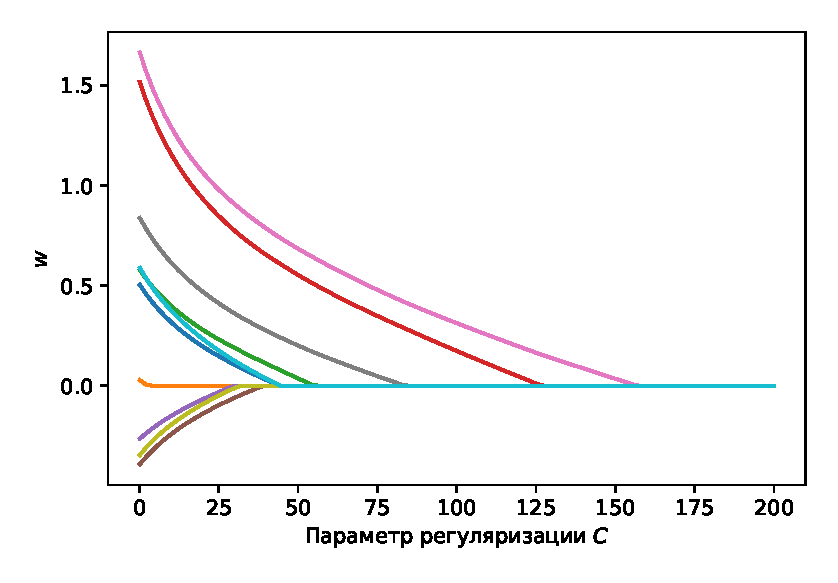
\includegraphics[width=0.5\textwidth]{../figures/log_reg_cs_exp.eps}
	\caption{Sample figure caption.}
	\label{fig:fig1}
\end{figure}

\subsection{Tables}
See awesome Table~\ref{tab:table}.

The documentation for \verb+booktabs+ (`Publication quality tables in LaTeX') is available from:
\begin{center}
	\url{https://www.ctan.org/pkg/booktabs}
\end{center}


\begin{table}
	\caption{Sample table title}
	\centering
	\begin{tabular}{lll}
		\toprule
		\multicolumn{2}{c}{Part}                   \\
		\cmidrule(r){1-2}
		Name     & Description     & Size ($\mu$m) \\
		\midrule
		Dendrite & Input terminal  & $\sim$100     \\
		Axon     & Output terminal & $\sim$10      \\
		Soma     & Cell body       & up to $10^6$  \\
		\bottomrule
	\end{tabular}
	\label{tab:table}
\end{table}

\subsection{Lists}
\begin{itemize}
	\item Lorem ipsum dolor sit amet
	\item consectetur adipiscing elit.
	\item Aliquam dignissim blandit est, in dictum tortor gravida eget. In ac rutrum magna.
\end{itemize}


\bibliographystyle{unsrtnat}
\bibliography{references}

\end{document}
